\documentclass[11pt]{article}

% Insert style guide
\usepackage{my_thesis}

% Specifiy the location of images to be used
\graphicspath{{figures/}}

%
\begin{document}
\title{\textsc{Nanoscopy using a semiconductor heterostructure as the sample stage}}
% \date{\footnote{Last Modified: \currenttime, \today.}}

% Create title page
\maketitle


\section{Abstract}
%
% Rewrite abstract mostly from the Xiaodong's feedback
A special structured illumination microscopy scheme using a two dimensional electron gas as the sample stage is proposed. Terahertz plasma waves generated by a current-driven instability illuminate the sample. Concurrently, a plane wave is used to shift the plasmonic pattern needed to expand the observable range of spatial frequencies. Full coverage of the spatial frequency regime is obtained by tuning the plasma waves through gate voltage control. Hence, it is possible to reconstruct an image with resolution up to two orders of magnitude beyond the diffraction limit. Due to the linear nature of the technique, only a weak illumination signal is required, therefore minimizing the likelihood of sample damage due to radiation.
%
\section{Introduction}
%
% As suggested by Xiaodong, discussion on confocal microscopy is unnecessarily long, and bloating this section. Trim it!
In conventional wide-field fluorescent microscopy, a sample is uniformly illuminated by a beam of light, and the resulting fluorescence is observed in the far-field through the objective lens. The uniform intensity of the illumination along the sample fundamentally restricts the resolution of the system to half the wavelength of light due to the Abbe diffraction limit. With ever growing need to image miniscule objects especially in life sciences, modern microscopy techniques such as confocal and linear structured illumination microscopy (SIM) use spatially non-uniform sources of light to illuminate the sample. This non-uniformity is directly attributed to obtaining resolution that can be extended beyond the diffraction limit by a factor of $2$ \cite{Minsky1988,Gustafsson2000}. Use of pinholes in confocal microscopy makes the technique highly inefficient as a significant part of light is discarded that may leave weakly fluorescent objects undetectable. Structured Illumination microscopy is a wide-field technique in which a fine illumination pattern such as a sinusoidal standing wave is used to generate \emph{Moiré fringes} in the
observed image \cite{Heintzmann1999, Heintzmann2006}. The high frequency content is mathematically reconstructed from a series of images acquired by shifting the pattern. Using a non-linear version of SIM, theoretically unlimited resolution can be achieved \cite{Gustafsson_2005}. However, high levels of illumination intensity are required, subjecting the sample to significant radiation damage.

Resolution beyond the classical diffraction by a factor greater than $2$ can be realized when an object is illuminated by surface waves, that are electromagnetic waves found at a material interface where one of the media possesses a complex dielectric function with a negative real part. The wavelength and phase velocity of the surface waves are much smaller than the homogeneous waves at the same frequency in a given medium. Using a grating structure to generate the surface waves with sub-diffraction features, a resolution with magnification factor of $20$ was first demonstrated at optical frequencies by Nassenstein \cite{Nassenstein1970}. Recently, a plasmonic structured illumination microscopy (PSIM) technique was proposed in which a sample was excited by surface plasmons existing at a metal-dielectric interface in the optical frequency range \cite{Wei2010}. In another scheme, it was shown that a hundred-fold resolution enhancement is possible using mid-infrared
graphene plasmons \cite{Zeng2014}.

Current-drive plasma instabilities have mainly been studied in the context of ionized gases \cite{9781489947871}.  An analagous activity leads to generation  of plasma waves in solid-state devices \cite{Kempa1991} that has led to many interesting applications in the far-infrared frequency region \cite{Dyer_2016, Wu2015}. A two-dimensional electron gas (2DEG) is formed at the interface of epitaxially grown semiconductors that acts as a transistor channel. In addition to the unusually high electron mobility, free-electron densities that are comparable to metals are observed without any intentional doping in the channel. Plasma waves originating in the electron channel of field-effect transistors which is only a few atoms thick were discovered more than 40 years ago \cite{Stern1967a, Allen1977} when excited by an external TM polarized plane wave. Field-effect transistor plasma waves have of late received great interest because of their application in engineering terahertz frequency sources and
sensors \cite{Dyakonov1993, Dyakonov1996, Popov2005, Otsuji2006, Dyakonov2005}. Although research has mainly been focused in realizing far-infrared devices, nitride based heterostructures have been used for the mid-infrared frequencies
\cite{Hofstetter2002}. More importantly, the frequency response of the device can be tuned by varying the gate voltage \cite{Fatimy2010, Rabbaa2011}.

In this paper, a nanoscale imaging technique is presented in which subwavelength plasma waves, generated by a current in a transistor channel that can be tuned by controlling gate voltage, are used as the illumination pattern required for SIM. The configuration effectively creates a much larger observable spatial frequency region as compared to a far-infrared (terahertz) plane wave. Due to the linear nature of the scheme, resolution of up to two orders of magnitude beyond the diffraction limit can be obtained with a weak field intensity. Although the wavelength is very small along the channel, it simultaneously brings the disadvantage of a fast decay in the vertical direction. The presence of a semiconductor layer above the channel further reduces the intensity of the wave. The resolution enhancement is ultimately limited by the layer thickness which should be kept as small as the fabrication process permits in order to reduce attenuation of the standing wave in the vertical direction.

%
\begin{figure}[t!]
  \centering
  \def\svgwidth{\linewidth}
  \input{figures/mstruc_gated.pdf_tex}
  \caption{Illustration of the imaging scheme where sample is excited by plasma wave pattern generated underneath by a current-driven instability}
  \label{fig:struct}
\end{figure}
%
%%%%%%%%%%%%%%%
%%%%%%%%%%%%%%%
%%%%%%%%%%%%%%%
%%%%%%%%%%%%%%%
%%%%%%%%%%%%%%%
%%%%%%%%%%%%%%%
%%%%%%%%%%%%%%%
%%%%%%%%%%%%%%%
%%%%%%%%%%%%%%%
\section{Theory}
\subsection{Dispersion relation}
%
A schematic diagram of the proposed system which is similar to a transistor, is shown in Fig. \ref{fig:struct} where a 2DEG that acts as a transistor channel is formed at the interface of two semiconductor materials of slightly different band-gap energies. Plasma waves are generated in the channel when the source and drain terminals are driven by a current source. Due to reflections from the conducting boundaries, the channel region forms a cavity in which the plasma waves form a standing wave. The structure is backed by a gate terminal that spans the length $L$ of the channel and spaced a distance $d$ below the 2DEG. The gate capacitively couples with the 2DEG, and by varying the voltage, the velocity as well as concentration of electrons in the channel can be controlled. A barrier layer of thickness $h$ separates the sample from the 2DEG.

The compressed nature of the plasma waves can be described by its dispersion relation. Here, we consider the sample stage which is terminated by a gate at the bottom and free-space at the top, excited by a $\mathrm{TM}$ polarized plane wave. The effects of the drain and source terminals are ignored by assuming the layered semiconductor structure along with the 2DEG channel to be of infinite lateral extent. The dispersion relation which shows a frequency dependent resonance response of plasma waves in the 2D channel, is obtained by imposing the transverse resonance condition realized by an equivalent transmission line (TL) circuit \cite{Kastner_1988,Michalski2005}. The 2DEG is modeled as a shunt admittance related to Drude-type surface conductivity \cite{Burke2000},
%
\begin{equation}
  Y_{\sigma} = \sigma_s = \frac{N_s e^2 \tau}{m^{\ast}}\frac{1}{1 + \j \O \tau},
  \label{eq:Y2deg}
\end{equation}
%
where $N_s$ is the surface electron density in the channel, $e$ is the electron charge, $m^{\ast}$ is the effective electron mass in the heterostructure, $\tau$ is the scattering time of electrons, and $\O$ is the angular frequency. The dispersion relation is then written as \cite{Gomez-Diaz2012}:
%
\begin{equation}
  Y^{\uparrow}(z_0) + Y^{\downarrow}(z_0) + Y_{\sigma} = 0.
  \label{eq:dispersion}
\end{equation}
%
Here, $Y^{\uparrow}(z_0)$ and $Y^{\downarrow}(z_0)$ are the up- and down-looking TL admittances from the 2DEG located at $z = 0$, and expressed as:
%
\begin{subequations}
  \begin{align}
    Y^{\uparrow}(z_0) &=  Y_2 \frac{1 - \Gamma^{\uparrow}(z_0)}{1 + \Gamma^{\uparrow}(z_0)},
    \label{eq:Yup} \\
    Y^{\downarrow}(z_0) &=  -\j Y_1 \cot (k_{z1} h).
    \label{eq:Ydown}
  \end{align}
  \label{eq:Y}%
\end{subequations}
%
For each layer, $Y_{i}$ and $k_{zi}$ where $i = 0,1,2$ are the respective TM mode admittance and transverse wavenumber of free-space, barrier and substrate layers respectively given by:
%
\begin{align}
  & Y_i = \frac{\O \E_i \E_0}{k_{zi}}, && k_{zi} = \pm \sqrt{k_0^2 \E_i - k_x^2}
  \label{eq:Yandk}
\end{align}
%
where $\E_i$ is the relative permittivity of $i^{\text{th}}$ layer and $k_x$ is the longitudinal propagation constant of the structure. The upward-looking reflection coefficient $\Gamma^{\uparrow}$ in \eqref{eq:Yup} is expressed in terms of the TM mode admittances:
%
\begin{equation}
  \Gamma^{\uparrow}(z_0) = \frac{Y_1 - Y_0}{Y_0 + Y_1} \e^{-2\j k_{z2}d_1}
  \label{eq:Gamma}
\end{equation}
%
% Structure details of GaN/ AlGaN
A closed-form expression for the longitudinal propagation constant $k_x$ by solving \eqref{eq:dispersion} is tedious, therefore numerical root-finding techniques such as the Newton method \cite{9780521880688} have to be employed. As an example, the dispersion diagram of a AlGaN/GaN heterostructure is shown in Fig. \ref{fig:dispersion} with no gate bias applied along with a light line whose slope is multiplied by a factor of 90 for illustration. The real part corresponds to propagation and imaginary part accounts for decay of the wave. The result is similar to a gated 2DEG plasmons in which the gate terminal is located at the top \cite{Nakayama1974, Eguiluz1975}. At \SI{25}{\THz}, the plasma wavenumber is approximately 80 times greater than that of free-space with negligible loss. Such extreme subwavelength phenomenon makes super-resolution possible. The structure parameters used to compute the dispersion relation via \eqref{eq:Y2deg}-\eqref{eq:Gamma} are now briefly discussed.

The gate-channel separation is $d = \SI{100}{\nm}$. The channel length $L$ is \SI{2}{\micm} whereas the AlGaN barrier layer is $h = \SI{20}{\nm}$ wide.
The permittivity of both semiconductor layers is approximated to the static value, i.e., $\E_1 \approx \E_2 = 9.5$ when the mole-fraction of aluminum in AlGaN alloy is taken as \SI{.2}{} \cite{Muravjov2010}. A surface carrier density of $N_s = \SI{5e13}{\cm^{-2}}$ and scattering time $\tau$ of \SI{114}{\ps} corresponding to a temperature of \SI{3}{\kelvin} is assumed. As the temperature is increased, $\tau$ gets smaller which leads to reduced mobility and introduces loss in the channel.
%
\begin{figure}[t!]
  \subfloat[]{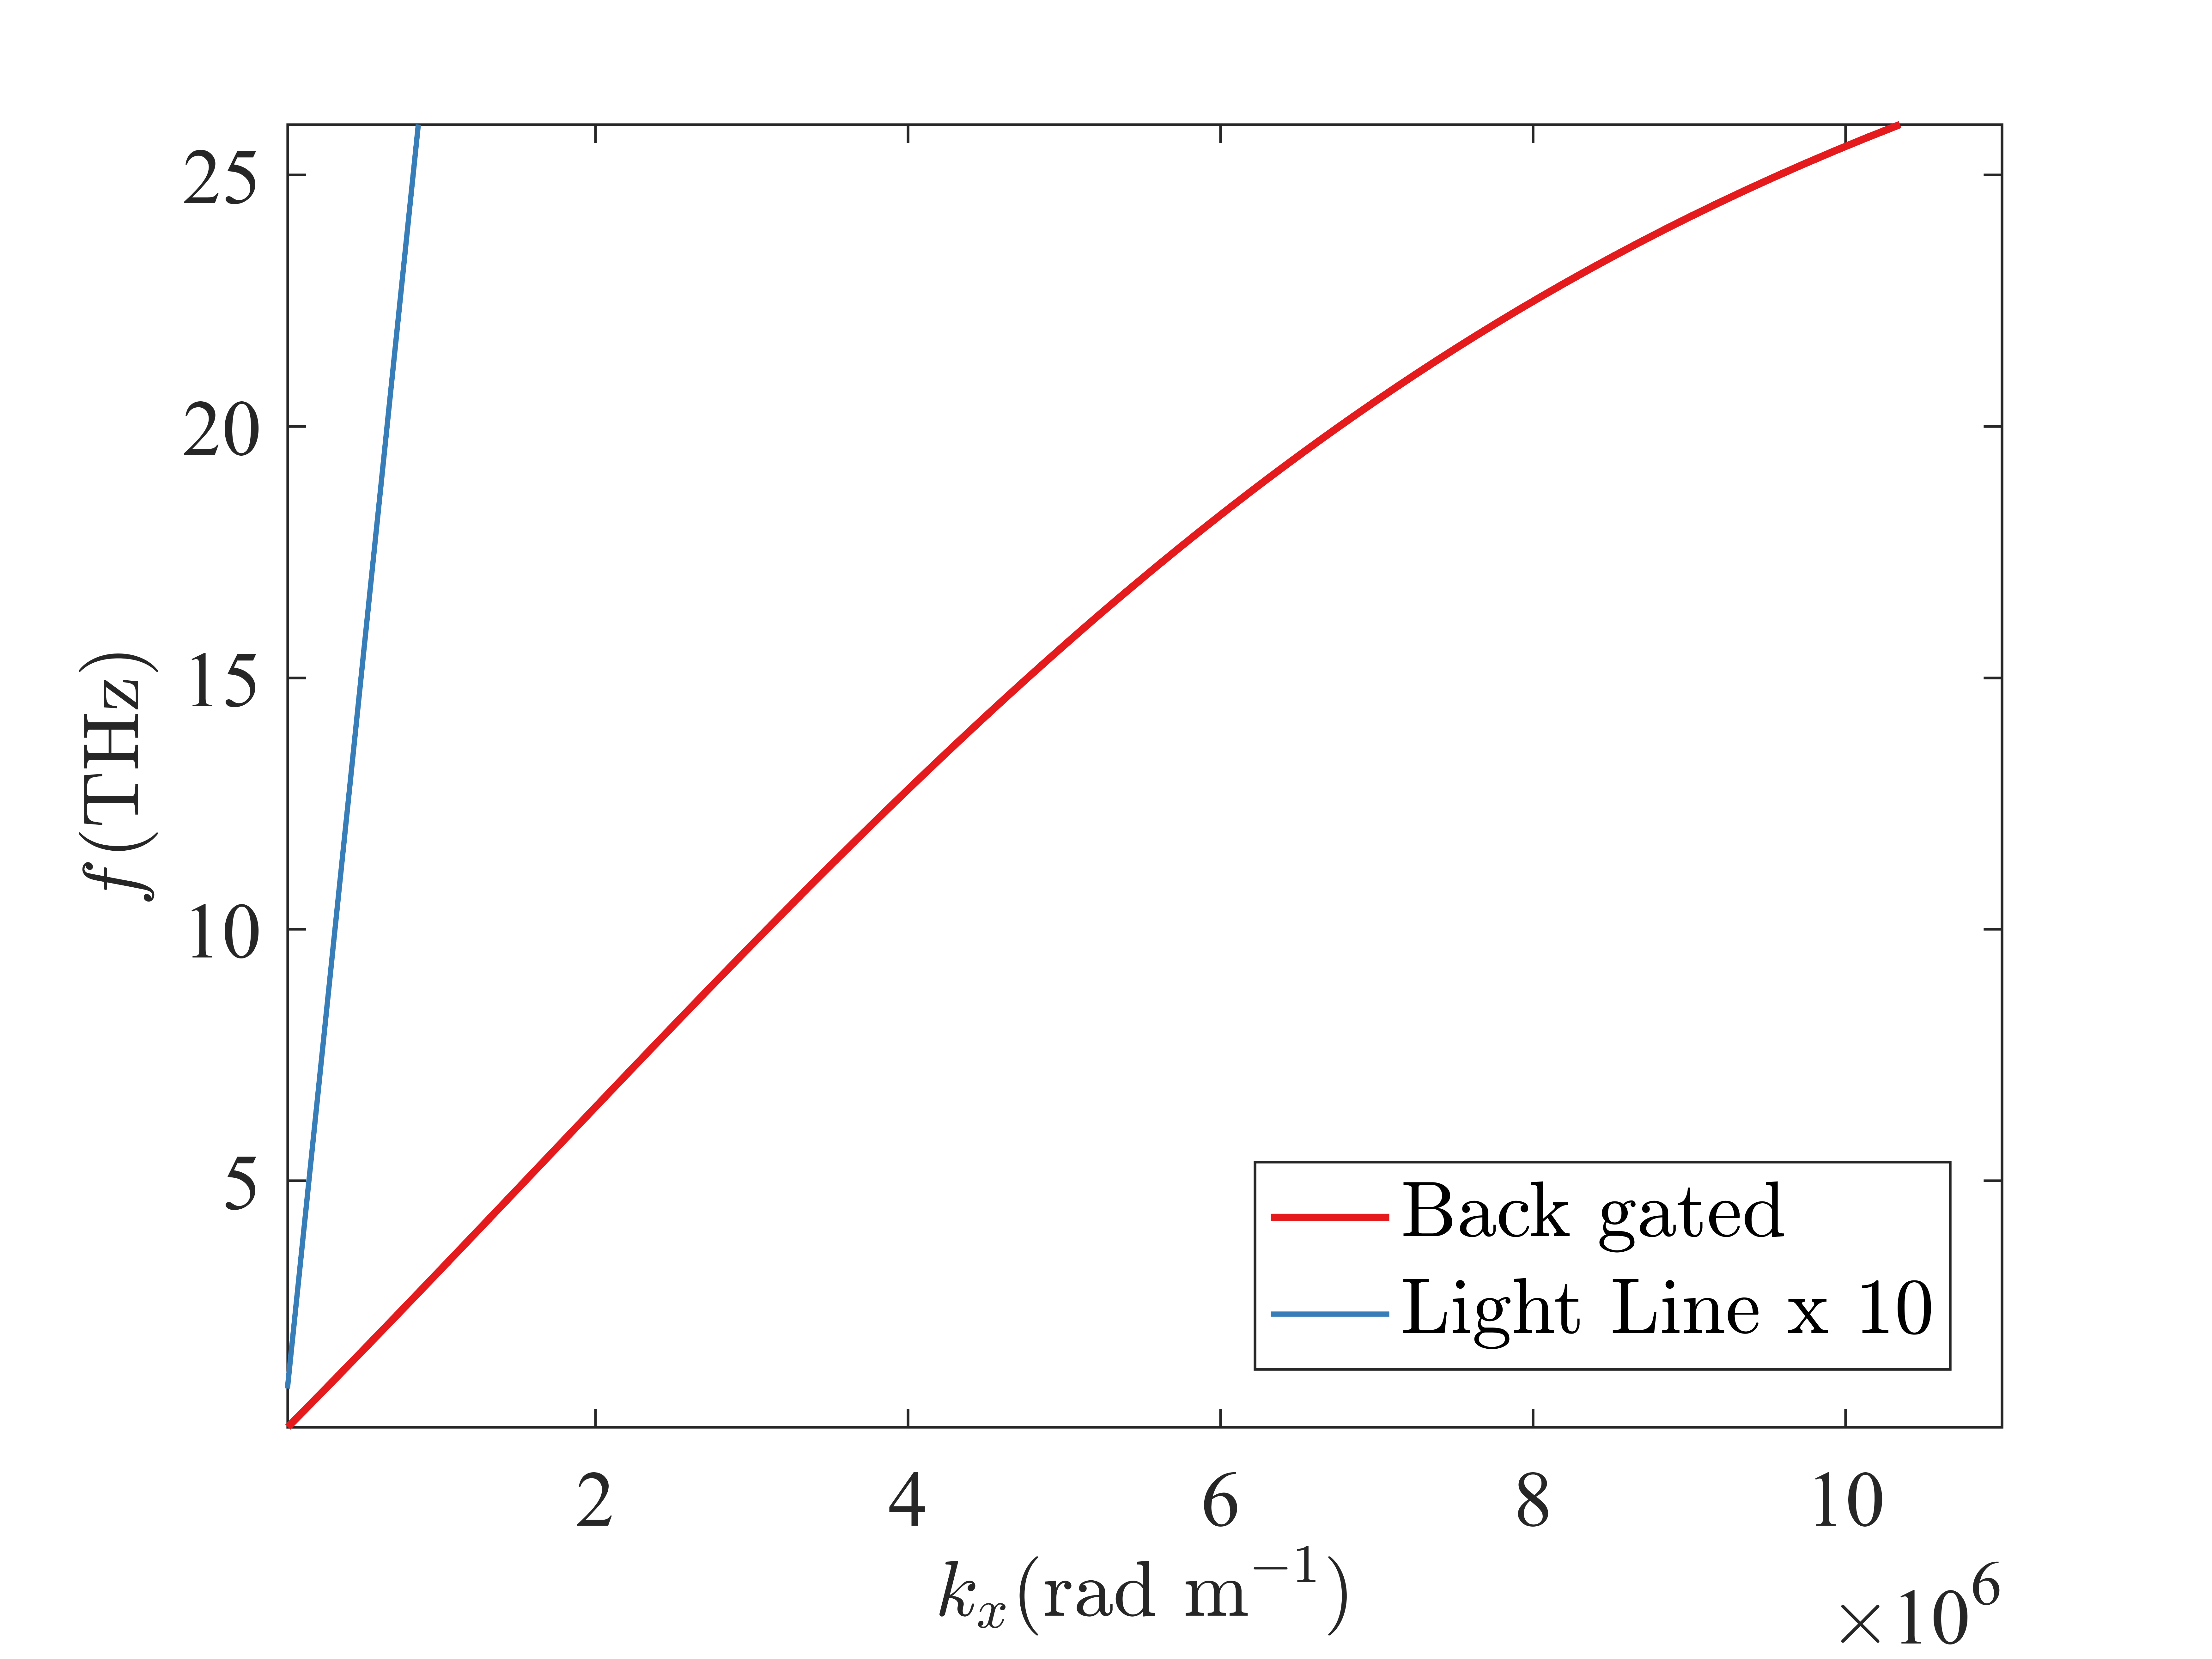
\includegraphics[height=2.5in]{gated_disp.tikz}
      \label{fig:dispersion}}
      \hfil
      \subfloat[]{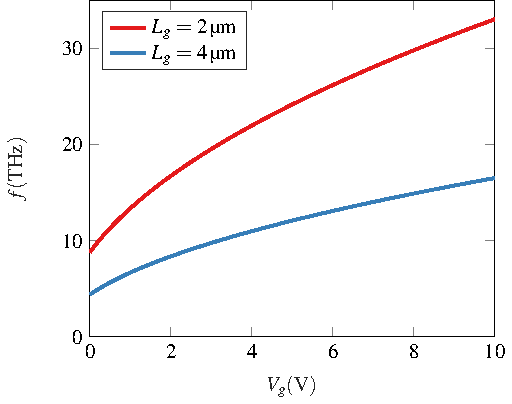
\includegraphics[height=2.5in]{gate_swing.tikz}
          \label{fig:tuning}}
  \caption{(a) Plasma wave Dispersion diagram for the transistor structure supporting a 2DEG channel. (b) Effect of gate voltage on resonant frequency}
  \label{fig:matlab_simulation}
\end{figure}
%
%% Now discuss tunability of the 2DEG
Through the gate voltage $V_g$, the electron density $N_s$ of the channel can be varied using:
%
\begin{equation}
  N_s = N_0 \times \left(1 - \frac{V_g}{V_T} \right),
  \label{eq:tunability}
\end{equation}
%
where $N_0$ is the zero-bias density and $V_T$ is the gate threshold voltage of the transistor. For a channel terminated by highly conducting source and drain terminals at each side, the resonant frequency as a function of carrier density is expressed as \cite{Popov2008}:
%
\begin{equation}
  \O = \sqrt{\frac{N_s \e^2 d}{m_{\ast} \E}} \frac{\pi}{L}
  \label{eq:plasma_frq}
\end{equation}
%
where $\E$ is the average permittivity of the surrounding media. Using \eqref{eq:tunability} and \eqref{eq:plasma_frq}, the tunability of plasma waves assuming a gate threshold voltage of \SI{-.764}{\volt} is shown in Fig. \ref{fig:tuning}. As expected, increasing the length of the channel reduces the resonant frequency.
%
%
%
\subsection{Image Reconstruction}
%
At low loss, the plasma wave illumination pattern $I(\v r)$ can be assumed sinusoidal and expressed as:
%
\begin{equation}
  I(\v r) = 1 + \cos(\v k_{\p} \cdot \v r + \phi)
  \label{eq:intensity}
\end{equation}
where $\v k_{\p} = k_x \v{\^{x}} + k_y \v{\^{y}}$ is the spatial frequency wavevector,  $\v r = x \v{\^{x}} +  y \v{\^{y}}$ is the two-dimensional positional vector and $\phi$ is the pattern phase. An image $M(\v r)$ of a sample atom distribution $F(\v r)$ observed through a microscope can be expressed as:
%
\begin{equation}
  M(\v r) = \left[ F(\v r) \cdot I(\v r) \right] \otimes H(\v r)
  \label{eq:m_spatial_image}
\end{equation}
%
where $H(\v r)$ is the point spread function (PSF) of the microscope, and $\cdot, \otimes$ denote multiplication and convolution operations in the spatial domain respectively. A frequency domain representation of the image obtained by taking the Fourier transform of \eqref{eq:m_spatial_image} is expressed as:
%
\begin{equation}
  \begin{split}
    \ti M(\v k) &= \left[ \ti F(\v k) \otimes \ti I(\v k) \right] \cdot \ti H(\v k) \\
     &= \frac{1}{2} \left[ 2\ti F(\v k) + \ti F(\v k - \v k_{\p}) \e^{- \j \phi} + \ti F(\v k + \v k_{\p}) \e^{\j \phi} \right] \cdot \ti H(\v k)
  \end{split}
  \label{eq:m_ft}
\end{equation}
%
where $\sim$ over the letters indicates a frequency domain term and $\ti H(k)$ is the optical transfer function (OTF) of the microscope. A spatial frequency representation of the scheme is illustrated in Fig. \ref{fig:sim}. Assuming a numerical aperture of (NA) of unity, the OTF can be described by a circular disc as shown in Fig. \ref{fig:sim}(a) where the passband is bounded by $\sqrt{k_x^2 + k_y^2} = \nu$. As evident in \eqref{eq:m_ft}, a sinusoidal illumination pattern has three frequency components which generates an image that is a linear combination of the sample along with two shifted versions as shown in Fig. \ref{fig:sim}(b). To reconstruct the sample, three different images need to be captured with each possessing a different phase term $\phi$. The process can be expressed as a system of linear equations,
%
\begin{equation}
  \ti H(\v k) \cdot
  \begin{bmatrix}
    \ti F(\v k) \\
    \ti F(\v k - \v k_{\p}) \\
    \ti F(\v k + \v k_{\p})
  \end{bmatrix}
  =
  \begin{bmatrix}
    2 & \e^{-\j \phi_1} & \e^{\j \phi_1} \\
    2 & \e^{-\j \phi_2} & \e^{\j \phi_2} \\
    2 & \e^{-\j \phi_3} & \e^{\j \phi_3} \\
  \end{bmatrix}^{-1}
  \begin{bmatrix}
   \ti M_1(\v k) \\
   \ti M_2(\v k) \\
   \ti M_3(\v k)
  \end{bmatrix}
  \label{eq:reconstruction_algo}
\end{equation}
%
\begin{figure}[t!]
  \centering
  \def\svgwidth{.75\linewidth}
  \input{figures/psim.pdf_tex}
  \caption{Resolution enhancement through SIM: (a) Diffraction limited observable region in frequency domain.  Moiré effect using a sinusoidal illumination pattern bringing high frequency content under the observable region. Sample illuminated at different plasma frequencies: (b)-(d). (e) Effective resolution enhancement of $k_{\p 1} + \upsilon$ in two dimensions can be obtained after rotating the sample with respect to the optical axis}
  \label{fig:sim}
\end{figure}
%
The phase shifts in \eqref{eq:reconstruction_algo} are known beforehand. Frequency content of the sample up to $k_{\p}$ can, therefore be observed due the Moiré effect which transports the high frequency information in to the observation region. To achieve two-dimensional enhancement in resolution, either the sample must be rotated about the optical axis of the microscope or the angular distribution of the illumination needs to be varied. The performance in terms of imaging speed can be improved by exciting the sample further with a pulse having energy higher than the plasmon illumination \cite{Zeng2015}. In the spatial frequency space, this corresponds to an enlarged OTF depicted by light-colored discs with radius $\upsilon$ in Fig. \ref{fig:sim}. Fewer tuned plasmon frequencies are therefore, required to achieve full coverage of the enlarged frequency region.
%
In order to laterally shift the pattern, an external TM polarized plane wave is used with an amplitude at least twice that of the plasma wave. The amount of shift is controlled by varying the angle of incidence with respect to the optical axis. Figure \ref{fig:shift} shows the lateral shift of the normalized plasma wave intensity at $z = h$ by changing the incident angle between \SI{-45}{\degree} and \SI{45}{\degree}. Because the plasmonic wavelength is much smaller than the channel length $L$, only a small portion of the channel is shown to illustrate the effect simulated using a full-wave commercial electromagnetic software \cite{comsol}.

%
% In this scheme, an external plane wave is used to shift the plasma wave pattern laterally in the sample stage. The electric field of a TM polarized plane wave is expressed as, $\v E_{ext} = \v{\^x} \, a  +  \v{\^z} \, b $. The total field at the surface is the sum of the plasmonic field and external plane wave. The total intensity is then expressed as:
% %
% % \begin{equation}
% %   \begin{split}
% %     \vert E \vert^2 &= (a + \cos k_{\p}x)^2 + (b + \sin k_{\p}x)^2 \\
% %     &=  a^2 + b^2 + 1 + 2 \chi \cos(k_{\p}x + \psi)
% %   \end{split}
% %   \label{eq:shift}
% % \end{equation}
%
% where $k_{\p}$ is the spatial frequency of plasma wave, $\chi = \sqrt{a^2 + b^2}$ and $\psi = \atan (b/a)$. The field components $a$ and $b$ are controlled by changing the incident angle of the plane wave. Using a commercial full-wave electromagnetic simulation tool \cite{comsol}, lateral shifting of the pattern is shown in Fig. \ref{fig:shift}. Since the wavelength is much smaller than the channel length, only a small portion is shown.  is As discussed earlier, the standing wave pattern can be tuned to different frequencies through gate voltage control.
Simulated standing wave patterns tuned to different frequencies by varying the gate voltage are shown in Fig. \ref{fig:s_waves}. The resulting change in electron density modifies the surface conductivity \eqref{eq:Y2deg} of the 2DEG and the dielectric function $\E(\O) = 1 - \j \sigma_s /(\O \Delta \E_r)$ where $\Delta$ is the 2DEG thickness.
%
\begin{figure}[t!]
  \subfloat[]{\includegraphics[height=2.8in]{figures/shifted1.tikz}
      \label{fig:shift}}
      \hfil
  \subfloat[]{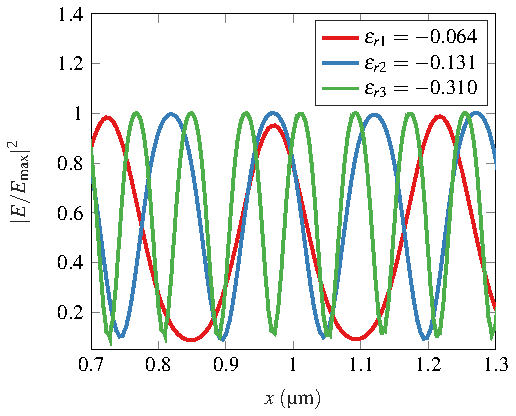
\includegraphics[height=2.8in]{tuning.tikz}
  \label{fig:s_waves}}
  \caption{Full-wave simulation results: (a) Phase shift achieved by exciting the structure with an external plane wave at an angle. (b) Tuning of the standing wave structure by applying gate bias}
  \label{fig:simulation1}
\end{figure}
%
%%%%%%%%%%%%%%%
%%%%%%%%%%%%%%%
%%%%%%%%%%%%%%%
%%%%%%%%%%%%%%%
%%%%%%%%%%%%%%%
%%%%%%%%%%%%%%%
%%%%%%%%%%%%%%%
%%%%%%%%%%%%%%%
%%%%%%%%%%%%%%%
\section{Simulated Results}
%
We consider a sample with atom distribution shown in Fig. \ref{fig:test}. Each particle shown has a diameter of \SI{1}{\nm}. The minimum separation between the atoms is \SI{38}{\nm} and maximum is \SI{137}{\nm}. The 2D plasma waves are generated by a dc current-driven instability that equivalently by excited by a TM polarized plane wave having frequency of \SI{25}{\THz}, $~h\O = \SI{.1}{\electronvolt}$ at zero gate bias. It is assumed that the numerical aperture (NA) is $1$. To demonstrate the super-resolution technique, the atom distribution is first Fourier transformed to the spatial frequency domain. The critical step to achieve super-resolution reconstruction involves computation of the inverse Fourier transform using frequency content up to a circular region of radius $2k_{\p} + \upsilon$, where $k_{\p}$ can be varied by gate voltage. In Figs. \ref{fig:sim_lo} and \ref{fig:sim_hi}, a resolution enhancement $39.5$ and $80$ is shown corresponding to \SI{152}{\nm} and \SI{74.9}{\nm} resolution respectively.
Figure. \ref{fig:sim_lo} shows that the particles that are separated by a distance less than the resolution can not be resolved and appear as a contiguous blurry streak, whereas they are distinguishable in Fig. \ref{fig:sim_hi}.
%
% Discuss loss in the scheme
% At cryogenic temperatures, the plasmons exhibit near loss-less behavior in the 2DEG where the real part of the wavenumber is at least three orders of magnitude greater than the imaginary part. However, as the temperature rises, the reduced electron mobility resulting due to electron scattering introduces a plasma wave decay factor such . To account for the loss, the plasma
%
\begin{figure}[t!]
  \subfloat[]{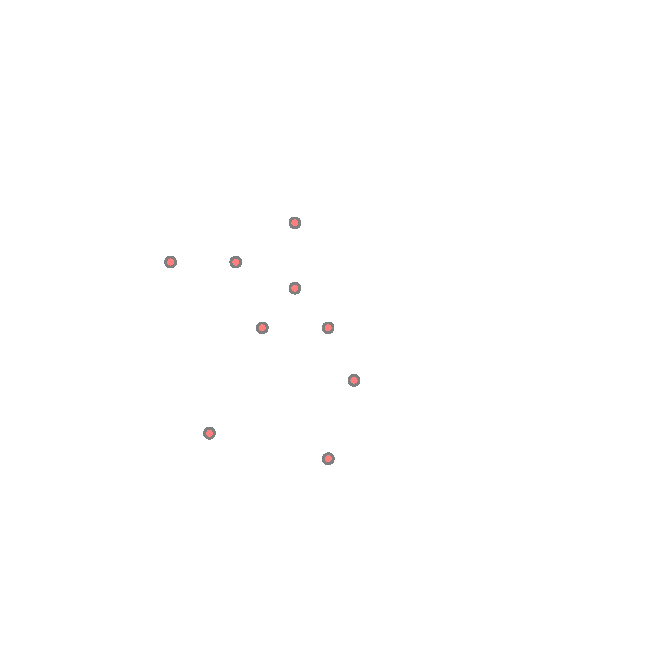
\includegraphics[height = 1.9in]{test_sample.tikz}
  \label{fig:test}} \hfil
  \subfloat[]{\includegraphics[height = 1.9in]{plsim_153.tikz}
  \label{fig:sim_lo}} \hfil
  \subfloat[]{\includegraphics[height = 1.9in]{plsim_75.tikz}
  \label{fig:sim_hi}}
  \caption{(a) Sample distribution. Simulation of the reconstructed sample image at: (b) $\Re k_{\p} = 39.5$ (c) $\Re k_{\p} = 80$}
  \label{fig:simulation}
\end{figure}
%%%%%%%%%%%%%%%
%%%%%%%%%%%%%%%
%%%%%%%%%%%%%%%
%%%%%%%%%%%%%%%
%%%%%%%%%%%%%%%
%%%%%%%%%%%%%%%
%%%%%%%%%%%%%%%
%%%%%%%%%%%%%%%
%%%%%%%%%%%%%%%
\section{Conclusion}
%
We propose a super-resolution nanoscopy scheme based on the subwavelength surface electromagnetic fields found in a semiconductor heterostructure. This method is useful in particular for light-sensitive samples as it requires a weak field intensity for illumination. The temperature dependent electron scattering introduces loss, which degrades the performance of the system with increase in temperature. The image reconstruction algorithm is as efficient as in conventional linear SIM, yet the high wave number along with tunability of the plasma waves allows it to achieve subdiffraction resolution of up to 80 times in the mid-infrared range.
%%%%%%%%%%%%%%%
%%%%%%%%%%%%%%%
%%%%%%%%%%%%%%%
\clearpage % Force Bibliography to the end of document on a new page.
% If using biber
% \printbibliography
% \addbibresource{zubairy}
% else bibtex
\bibliography{zubairy}
\bibliographystyle{ieeetran}

\end{document}
